%=============================================================================
%  MediMatrx - IEEE conference format report
%  Cloud Computing (DV2626), Blekinge Institute of Technology
%
%  HOW TO USE IN OVERLEAF
%    1. overleaf.com -> New Project -> Upload Project
%    2. Upload the zip containing this file and architecture-diagram.pdf
%    3. Menu -> Compiler -> pdfLaTeX
%    4. Recompile
%
%  IEEEtran.cls ships with Overleaf, so nothing needs installing.
%=============================================================================
\documentclass[conference]{IEEEtran}
\IEEEoverridecommandlockouts

\usepackage{cite}
\usepackage{amsmath,amssymb}
\usepackage{graphicx}
\usepackage{textcomp}
\usepackage{xcolor}
\usepackage{booktabs}

% [hyphens] lets long URLs break across lines instead of overflowing the column.
\usepackage[hyphens]{url}
\Urlmuskip=0mu plus 1mu   % let URLs stretch instead of overflowing
\usepackage{array}
\newcolumntype{L}[1]{>{\raggedright\arraybackslash}p{#1}}

\begin{document}

\title{MediMatrx: A Microservice Architecture for\\
Hospital Electricity Cost Optimisation with\\
Guaranteed Clinical Load Protection}

\author{\IEEEauthorblockN{Abhinav Annareddy}
\IEEEauthorblockA{\textit{Department of Computer Science} \\
\textit{Blekinge Institute of Technology}\\
Karlskrona, Sweden \\
aban24@student.bth.se}
}

\maketitle

%=============================================================================
\begin{abstract}
Swedish electricity is priced hourly on a day-ahead market, and within a single
day the spread between the cheapest and most expensive hour is commonly a factor
of three. A large regional hospital spends roughly 8--15 MSEK a year on power,
and although it cannot reduce what it consumes, a useful share of that
consumption can be moved in time. This report describes MediMatrx, an
application that plans such a move and reports what it is worth, while
guaranteeing that patient-critical load is never touched. The system runs as ten
microservices across two tiers, plus a document database, on Kubernetes,
reachable from a browser through a single gateway; four of the ten services
handle authentication, verification, input validation and authorization, and
six handle the energy-optimisation domain itself. Two aspects are treated in
detail. The first is the decomposition, which follows how the components scale
rather than how the code is organised, and places the business logic in exactly
one service. The second is the placement algorithm, which went through three
versions: the first raised the site peak by 938 kW while reporting a reduction
of zero, the second fixed that but cut the energy saving to 1.9\%, and only the
third handles both tariff components at once. Measured over twelve runs on live
market data, the deployed system reduces the daily energy bill by 11.4\% and
cuts site peak demand by a median of 423 kW.
\end{abstract}

\begin{IEEEkeywords}
microservices, Kubernetes, cloud architecture, demand-side management, energy
optimisation, REST, containerisation
\end{IEEEkeywords}

%=============================================================================
\section{Introduction}

Electricity in the Nordic area is traded a day ahead and settled by the hour. In
Swedish bidding area SE4 the cheapest hour of an ordinary day costs about a
third of the dearest one. Any consumer able to schedule some of its load can
therefore spend less without consuming less, purely by choosing when the work
happens.

Hospitals are a good candidate for this and an awkward one. They are large
consumers, they never close, and a fair share of what they use is schedulable:
laundry, sterilisation, catering, and the ventilation plant, which can be run
early because the building itself stores the result. The awkward part is the
rest. Intensive care, operating theatres, imaging and inpatient wards are
life-safety loads, and no price signal justifies delaying them. So the first
design question is not how to save money. It is where to put the boundary
between the two kinds of load, and how to stop anything crossing it.

I built MediMatrx to answer that question and, at the same time, to serve as a
worked example of provisioning and deploying a microservice system. The report
covers four things: the decomposition and why it is drawn where it is
(Section~\ref{sec:arch}); the two-tier arrangement that keeps the business logic
in one place (Section~\ref{sec:tiers}); the placement algorithm, including the
two versions that were wrong (Section~\ref{sec:algorithm}); and the Kubernetes
deployment (Section~\ref{sec:deploy}).

%=============================================================================
\section{Application Description}

\subsection{Load classification}

The hospital is modelled as nine metered zones in three classes.

\emph{Clinical.} Intensive care, operating theatres, imaging and inpatient
wards. Never shifted, reduced or delayed. The exclusion lives in the optimiser,
not in the interface, so there is no sequence of clicks that can defeat it.

\emph{Deferrable.} Ventilation and chiller plant, sterilisation, laundry and
catering. The work still happens every day; only its timing is open. Each zone
has a shiftable fraction taken from how the equipment actually behaves. Laundry
is 0.85, since an industrial wash can be run overnight provided it is finished
before the morning round. Ventilation is only 0.30, because the flexibility
comes from the building's thermal mass and that runs out.

\emph{Fixed.} Administration, which follows office hours and is left alone.

\subsection{What the system does}

Six things. It stores meter readings; fetches live hourly prices; computes a
shifting plan and reports the money, peak and carbon involved; flags hours where
a zone drew far more power than the hours either side, which usually means a
chiller is short-cycling or a damper is stuck; answers questions typed in
English using figures pulled from its own APIs; and predicts tomorrow's load
from the weather forecast so it can plan a day that has not happened yet.

The first five describe the past. Only the sixth produces something an estates
manager can act on when they arrive in the morning, which is the difference
between a dashboard and a tool.

\subsection{Scale, acknowledged}

One hospital does not need any of this to scale. A single replica of each
service would carry the load without difficulty, and I would rather say so than
pretend otherwise. The scaling argument only becomes real if the system is run
as a service for a group of hospitals. At that point the three workloads pull
apart: ingest grows with the number of meters installed, the optimiser grows
with the number of sites being replanned, and the price service does not grow at
all, because every customer in a bidding area sees the same prices. Three
different growth curves is the reason they are three different services.

For the demonstration to make sense, read the nine zones as nine hundred zones
across sixty hospitals, with every site replanned each time new price data
arrives.

%=============================================================================
\section{Architecture}
\label{sec:arch}

\begin{figure*}[t]
\centering
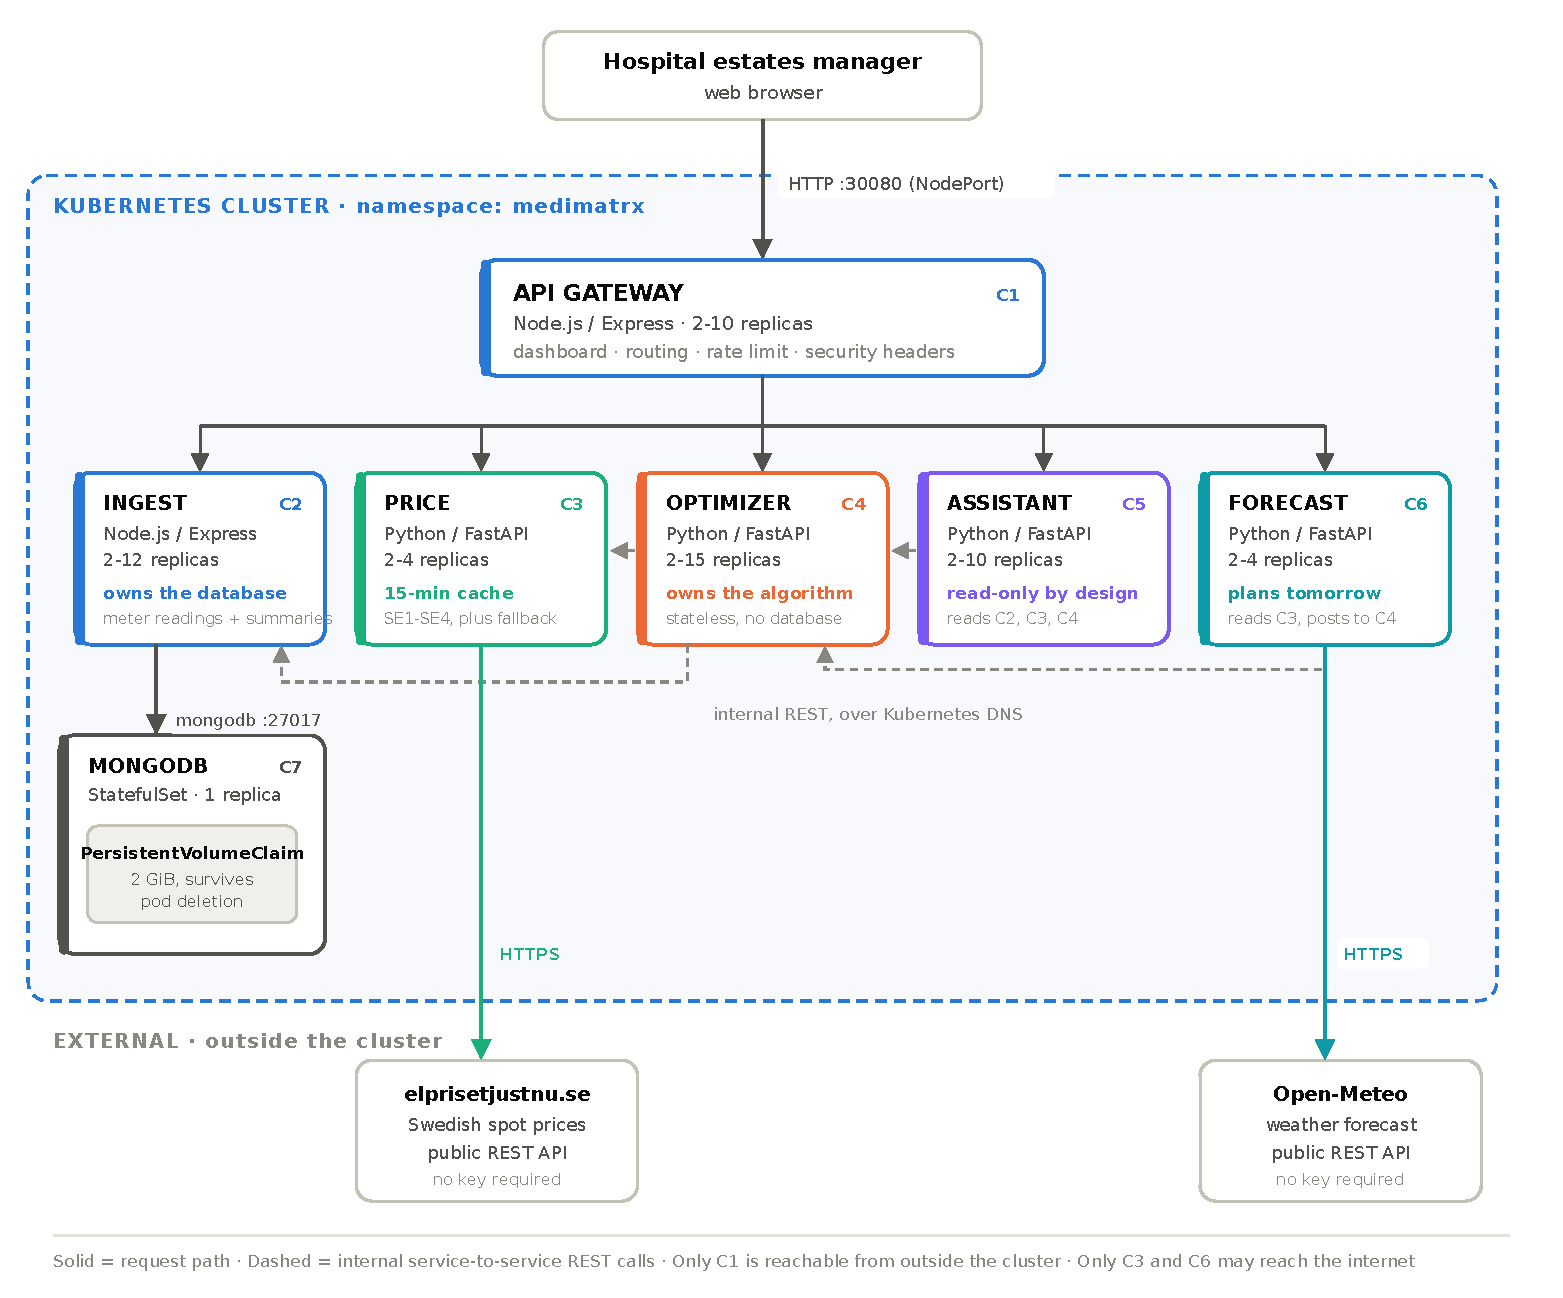
\includegraphics[width=0.92\textwidth]{architecture-diagram.pdf}
\caption{Component and deployment architecture. C1--C11 are the logical
components mapped in Table~\ref{tab:mapping}. Solid arrows show the request
path, dashed arrows internal REST calls between services. Only C1 is reachable
from outside the cluster, and only C3 and C6 may reach the public internet.}
\label{fig:arch}
\end{figure*}

\subsection{Two tiers}
\label{sec:tiers}

Fig.~\ref{fig:arch} shows the system split into two tiers. Tier 1 services each
own something: the meter data, the identity data, the price cache, or the
optimisation algorithm. Tier 2 services own nothing. The assistant and forecast
services answer questions and build plans by calling Tier 1; the verification,
validation and authorization services each answer one narrow identity question
by consulting Tier 1's auth service or their own signing secret. Either way,
there is one copy of the algorithm and one copy of every kind of data in the
whole system.

The forecast service is where this matters. It could easily have held its own
copy of the optimisation routine, and an earlier sketch did. Instead it posts
the day it has predicted to the optimiser's scenario endpoint and gets a plan
back. Today's report and tomorrow's plan therefore come out of the same code and
cannot disagree. Features of this kind usually fail when the live view and the
predictive view drift apart over a few months of changes, and the drift is
invisible until a customer notices. Removing the second copy removes the failure
mode rather than managing it.

\subsection{Components and the services that implement them}

Table~\ref{tab:mapping} gives the mapping the assignment asks for.

\begin{table*}[t]
\caption{Mapping of logical components to microservices}
\label{tab:mapping}
\centering
\begin{tabular}{@{}clL{3.1cm}L{2.6cm}L{2.3cm}L{3.4cm}@{}}
\toprule
\textbf{\#} & \textbf{Tier} & \textbf{Logical component} & \textbf{Service} &
\textbf{Runtime} & \textbf{Owns state?} \\
\midrule
C1 & --- & Presentation and entry point & \texttt{gateway} & Node.js 20 / Express & No \\
C2 & 1 & Metering data management     & \texttt{ingest}    & Node.js 20 / Express & Yes, owns MongoDB \texttt{readings} \\
C3 & 1 & Market price acquisition     & \texttt{price}     & Python 3.12 / FastAPI & In-memory cache only \\
C4 & 1 & Optimisation and analytics   & \texttt{optimizer} & Python 3.12 / FastAPI & No, fully stateless \\
C5 & 2 & Natural-language explanation & \texttt{assistant} & Python 3.12 / FastAPI & No, fully stateless \\
C6 & 2 & Next-day prediction          & \texttt{forecast}  & Python 3.12 / FastAPI & No, fully stateless \\
C7 & 1 & Identity and credentials     & \texttt{auth}      & Python 3.12 / FastAPI & Yes, owns MongoDB \texttt{users}, \texttt{verification\_codes} \\
C8 & 2 & One-time verification codes  & \texttt{verification} & Python 3.12 / FastAPI & No, delegates to C7 \\
C9 & 2 & Input validation             & \texttt{validation}   & Python 3.12 / FastAPI & No, fully stateless \\
C10 & 2 & Authorization               & \texttt{authorization} & Python 3.12 / FastAPI & No, fully stateless \\
C11 & --- & Persistence                & \texttt{mongodb}   & MongoDB 7.0 & Yes \\
\bottomrule
\end{tabular}
\end{table*}

\textbf{C1, API Gateway.} The only public entry point. It serves the dashboard
and routes API calls, and it is where the cross-cutting work happens once
instead of nine times: security headers, rate limiting, request logging, upstream
timeouts. Without it the browser would need nine addresses and all nine backend
services would need exposing.

\textbf{C2, Ingest.} Owns the \texttt{readings} collection. Nothing else has
credentials for it, and a NetworkPolicy blocks the connection independently of
whether anything else does.

\textbf{C3, Price.} A client of somebody else's REST API and a server of its
own. It normalises whatever comes back into 24 hourly values and caches for
fifteen minutes. If the upstream fails it serves the stale cache; if there is no
cache it serves a modelled curve, labelled as modelled.

\textbf{C4, Optimizer.} The business logic, covered in
Section~\ref{sec:algorithm}. CPU-bound and stateless, which makes it the easiest
thing here to scale and the first thing that will need it.

\textbf{C5, Assistant.} Turns a question in English into an answer. This is the
one service where a wrong answer would not look wrong: everything else returns
JSON that is either right or visibly broken, whereas fluent prose reads the same
whether or not it is true. Keeping it separate lets the rule be stated exactly
and then checked, and the rule is that the assistant does no arithmetic. Every
figure it quotes was fetched from another service during that request. It holds
no database credentials and no write path, so no phrasing of any question can
change hospital data. An optional language model may reword an answer that has
already been computed; if it is absent or fails, the deterministic answer is
served unchanged, which is why the demonstration needs no API key.

\textbf{C6, Forecast.} Fetches the weather forecast, converts it to predicted
per-zone load through a degree-hour model, gets tomorrow's prices from C3 and
asks C4 for a plan. Each plan carries a confidence rating and its caveats,
because tomorrow's day-ahead prices do not exist until the market publishes them
in the early afternoon. Before that the service says so instead of presenting a
model output with the same confidence as a measurement.

\textbf{C7, Auth.} Registers accounts, checks credentials, issues signed JWTs,
and is the sole owner of the \texttt{users} and \texttt{verification\_codes}
collections. On registration it asks C8 to mint a one-time code and C8 calls
back to a token-gated internal endpoint on C7 to store it, so C7 stays the only
writer of its own collections.

\textbf{C8, Verification.} Issues and checks one-time account codes without
keeping a copy of the account itself; every replica agrees with the one real
record in C7's database because it holds no data of its own.

\textbf{C9, Validation.} Checks a meter reading or a registration is
well-formed before it reaches C2 or C7. Called by the gateway before it
forwards a write; rejects with a 400 and a list of errors on failure.

\textbf{C10, Authorization.} Decodes the JWT C7 issued and checks the caller's
role against the action attempted. Called by the gateway before every
protected proxy call; a \texttt{staff} account may read and write, a
\texttt{viewer} account may only read.

\textbf{C11, MongoDB.} One shared instance, service-owned collections rather
than one database per service. Meter readings and identity records are both
schemaless documents, written far more than updated and read back through
aggregations or single-key lookups, so a document store suits both without a
migration every time a new meter type or account field appears.

\subsection{Patterns}

Table~\ref{tab:patterns} lists the patterns \cite{richardson2018,newman2021,
fowler2014} used to connect the components.

\begin{table}[t]
\caption{Cloud architecture patterns employed}
\label{tab:patterns}
\centering
\begin{tabular}{@{}L{2.5cm}L{5.2cm}@{}}
\toprule
\textbf{Pattern} & \textbf{Why it is here} \\
\midrule
API Gateway & One public entry point; cross-cutting concerns applied once. \\
Service-Owned Collections & Only \texttt{ingest} and \texttt{auth} may reach MongoDB, each restricted to its own collections, enforced by credentials and by NetworkPolicy. \\
Backend for Frontend & The browser sees one same-origin API; internal boundaries can move. \\
Service Discovery & Kubernetes DNS; no IP address appears in code or config. \\
Cache-Aside & Turns hundreds of calls on a third-party API into four an hour. \\
Graceful Degradation & An upstream outage costs one value's accuracy, not the dashboard. \\
Retry with Backoff & Start-up order is not guaranteed, so \texttt{ingest} waits instead of crash-looping. \\
Health/Readiness Separation & Liveness failure restarts a pod; readiness failure only takes it out of rotation. \\
Grounded Assistant & The service that writes sentences is not allowed to do arithmetic. \\
Single Source of Truth & \texttt{forecast} posts scenarios to C4 rather than reimplementing it. \\
\bottomrule
\end{tabular}
\end{table}

\subsection{One request, end to end}

Loading the dashboard sends a request to the gateway, which forwards it to an
optimiser replica. That replica fetches consumption from ingest and prices from
the price service at the same time rather than one after the other, so two
200~ms calls take 200~ms. The ingest replica runs a MongoDB aggregation to
produce the per-zone hourly matrix; the price replica returns a cached or
freshly fetched curve. The response names every pod that took part, which is how
the scaling demonstration is made visible rather than asserted.

%=============================================================================
\section{The Optimisation Algorithm}
\label{sec:algorithm}

I have written this section out in full, including the parts that did not work,
because the two failures are more informative than the final design.

\subsection{Two bills}

A Swedish hospital pays for electricity twice. There is energy, in kWh, priced
by the hour. There is also a grid demand charge (\emph{effektavgift}), billed on
the single highest hour of the month. An algorithm that optimises one of these
and ignores the other can be arithmetically correct and still cost the customer
money.

The model uses 34 SEK/kW/month. That is the top of Vattenfall Eldistribution's
base band for high-voltage business subscriptions \cite{vattenfall2025}, which
runs 11--34 SEK/kW/month; Sk\aa nska Energi charges 265 SEK/kW/year, about 22
SEK/kW/month \cite{skanska2026}. Vattenfall additionally levies a high-load
surcharge of 21--86 SEK/kW/month in January, February, March, November and
December, which this model ignores entirely. The demand-side figures reported
here are therefore conservative for a customer on that tariff.

\subsection{First version: greedy, per zone}

The first implementation took a shiftable fraction out of each expensive hour
and refilled the cheapest hours first, capping each receiving hour at 1.6 times
the zone's typical load. The cap was per zone. Nothing looked at the site
total.

Every deferrable zone therefore picked the same cheapest hour, and between them
they built a new peak higher than the one just removed. On live data the site
peak went from 1943 kW to 2881 kW. The reported figure was computed as
$\max(\Delta,0)$, so the dashboard displayed ``0 kW'' --- a 938 kW regression
shown as a neutral result. Of the two mistakes, the clamp was the worse one.

\subsection{Second version: water filling to the lowest ceiling}

Placement was split into two passes. In the first, every zone releases its
movable load and nothing is placed. In the second, the site profile after
removal is known, so load is placed up to a site-wide ceiling $C$, cheapest hours
first, with no hour allowed above $C$. This is water filling, the usual way of
posing peak minimisation: $C$ is the smallest value satisfying

\begin{equation}
\sum_{h \in H} \max\!\left(C - p_h,\; 0\right) \;\ge\; E
\label{eq:waterfill}
\end{equation}

where $p_h$ is the post-removal load in hour $h$, $H$ the candidate placement
hours, and $E$ the energy released. The left side is monotone in $C$, so binary
search finds it.

Splitting the passes is what makes the second one possible at all. Where load
lands is a decision about the whole site, and it cannot be taken one zone at a
time.

Letting $H$ contain all twenty-four hours also buys a guarantee. The hospital's
actual profile is itself a valid arrangement that fits under its own peak, so
$C$ equal to the baseline peak is always feasible and the search can never
return more. The optimiser cannot increase site peak demand. That follows from
the method; it is not a case that is tested for and patched.

This version removed the peak defect and introduced a different one. Taking the
\emph{lowest} feasible ceiling fills the cheap hours completely, so everything
placed after that has to go somewhere dearer. Measured on live SE4 data: peak
reduction 469 kW, energy saving down to 1.9\%, and the zones placed last being
told to run during the evening price peak at a loss. Some individual
recommendations carried negative values. The dashboard was advising the user to
move laundry into the most expensive window of the day.

\subsection{Third version: choosing the ceiling by what it is worth}

The current design searches for the ceiling instead of assuming one. Forty-one
candidates are evaluated between the minimum feasible ceiling and the baseline
peak, and each resulting plan is priced on both bills:

\begin{equation}
V(C) = 365\,\big(B_e - E(C)\big) \;+\; 12\,\tau\,\big(P_b - P(C)\big)
\label{eq:value}
\end{equation}

with $B_e$ the baseline daily energy cost, $E(C)$ the optimised cost, $P_b$ and
$P(C)$ the baseline and optimised peaks, and $\tau$ the demand charge in
SEK/kW/month. The plan with the highest $V$ is returned. Placement is
$O(|Z|\cdot 24)$ for $|Z|$ zones, so forty-one of them cost microseconds, and
searching removes a trade-off that would otherwise need retuning for every price
curve.

\subsection{How results are reported}

Two rules follow from the above.

The peak change is reported signed. A plan that raises the peak has to be shown
raising it.

If the energy bill would rise by more than the demand charge falls, the plan is
not recommended. This happens on inverted days, when cheap power arrives during
the site's busiest hours. The interface then leads with ``change nothing today''
and shows the net loss. Claiming a saving on a day when there is none is worse
than saying nothing, because somebody acts on it.

%=============================================================================
\section{Deployment}
\label{sec:deploy}

\subsection{Kubernetes objects}

61 resources across 15 manifests, validated against the upstream API schemas
with \texttt{kubeconform --strict}: a Namespace, a ConfigMap and two Secrets, a
StatefulSet with a \texttt{volumeClaimTemplate}, ten Deployments with their
Services, ten HorizontalPodAutoscalers, nine PodDisruptionBudgets and 16
NetworkPolicies (a default-deny-all plus 15 explicit allows). Every image is
published to Docker Hub so the scheduler can pull it on any node.

\subsection{Independent scaling}

Each service has its own HorizontalPodAutoscaler with its own metric, target and
bounds (Table~\ref{tab:hpa}). Nothing is shared between them, so nothing couples
their behaviour.

\begin{table}[t]
\caption{Autoscaling configuration}
\label{tab:hpa}
\centering
\begin{tabular}{@{}lccL{3.4cm}@{}}
\toprule
\textbf{Service} & \textbf{Min} & \textbf{Max} & \textbf{Scaling signal} \\
\midrule
\texttt{gateway}   & 2 & 10 & CPU 60\%; grows with concurrent users \\
\texttt{ingest}    & 2 & 12 & CPU 65\% and memory 75\%; grows with meter count \\
\texttt{price}     & 2 & 4  & CPU 70\%; capped on purpose \\
\texttt{optimizer} & 2 & 15 & CPU 55\%; stateless computation \\
\texttt{assistant} & 2 & 10 & CPU 60\%; grows with users, not meters \\
\texttt{forecast}  & 2 & 4  & CPU 65\%; capped on purpose \\
\texttt{auth}      & 2 & 8  & CPU 65\%; login/registration traffic \\
\texttt{verification} & 2 & 8 & CPU 65\%; stateless, cheap per call \\
\texttt{validation}   & 2 & 12 & CPU 65\%; on the critical path of every write \\
\texttt{authorization} & 2 & 10 & CPU 60\%; called on every protected request \\
\bottomrule
\end{tabular}
\end{table}

The low ceilings on \texttt{price} and \texttt{forecast} are a decision, not an
omission. Each replica keeps its own cache, so adding replicas increases the
load placed on a third-party API while lowering the hit rate. What a service
depends on sets its ceiling, not how much traffic one would like it to take.

Scale-up and scale-down are asymmetric on purpose: react immediately when load
arrives, contract over a 180--300 second window, so a short lull does not make
replicas thrash.

\subsection{Persistent storage}

MongoDB runs as a StatefulSet with a \texttt{volumeClaimTemplates} entry
requesting 2 GiB \texttt{ReadWriteOnce}. That creates a PersistentVolumeClaim
which is not deleted when the pod is. \texttt{storageClassName} is left out
deliberately so the cluster's default class applies: \texttt{hostpath} on Docker
Desktop, \texttt{standard} on Minikube, a cloud block device on a managed
cluster. The same manifest deploys in all three. Deleting the pod and watching
the readings survive is the demonstration.

%=============================================================================
\section{Benefits and Challenges}

\subsection{Benefits}

Each component scales on its own driver, which is the argument made in
Section~\ref{sec:arch}. Runtimes can differ: Node.js for the I/O-bound gateway
and ingest, Python for the computational services, without either choice
constraining the other. Failures stay local, so losing the price upstream costs
one number rather than the page. And the safety rule sits in one file, which is
what makes it auditable by somebody whose job is clinical safety rather than
software.

\subsection{Challenges and what was done}

\emph{Debugging across processes.} One optimisation request becomes three
network hops and no stack trace spans them. Every service emits single-line
structured JSON tagged with service and pod, and each response carries the
identity of every pod that answered.

\emph{Stale prices.} Prices can be fifteen minutes old. The market settles
hourly, so this is tolerable, and the age is shown next to the data.

\emph{One database pod.} A real weakness, accepted because the assignment states
the database need not scale. In production this would be a three-member replica
set with restores that have actually been tested.

\emph{Rate limiting per pod.} The counter lives in one pod's memory, so with $n$
replicas the real limit is $n$ times the configured one. The fix is Redis, or
limiting at the ingress.

\emph{Operational weight.} Sixty-one Kubernetes objects and ten images need a
build pipeline and somebody on call. For one hospital that is a bad trade, and
it only becomes reasonable across many sites.

%=============================================================================
\section{Security}

\subsection{What was done}

\emph{One way in.} Only the gateway has a NodePort, on port 30080. The other nine services are
ClusterIP and have no address reachable from outside.

\emph{Default-deny networking.} Kubernetes lets every pod talk to every other
pod unless told otherwise. A \texttt{default-deny-all} policy reverses that, and
15 further policies (16 NetworkPolicy objects in total) then open only what is
needed. The important one is \texttt{mongodb-ingress}: only pods labelled
\texttt{app: ingest} or \texttt{app: auth} may open a TCP connection to the
database, so an attacker holding the database password from a compromised
optimiser pod would still be refused by the network. Egress is
handled the same way. Only \texttt{price} and \texttt{forecast} may reach the
internet, only on 443, with RFC 1918 ranges excluded, so neither can be turned
into a scanner for the internal network.

\emph{Least privilege in containers.} Non-root user, no privilege escalation,
all Linux capabilities dropped, read-only root filesystem. A compromised process
cannot write a payload to disk.

\emph{Input and output handling.} Request bodies are validated by pydantic
models with explicit bounds, everything rendered into the dashboard is
HTML-escaped, and the gateway sets a Content-Security-Policy and four further
headers.

\emph{Injection.} Queries go through the driver's document API rather than
string building, and the assistant has no write path at all.

\subsection{What was done: identity}

Every \texttt{/api} route but registration, verification and login requires a
bearer token, checked by a dedicated \texttt{authorization-service} before the
gateway proxies anywhere. Authentication and authorization are split across two
services on purpose: a permissions change should never require touching the
code that checks a password, and vice versa. \texttt{auth-service} is the sole
owner of the two MongoDB collections holding identity data; the
\texttt{verification-service} that issues and checks one-time codes holds no
data of its own, so it stays horizontally scalable with no shared cache. A
\texttt{staff} account may read and write; a \texttt{viewer} account is
read-only, enforced server-side rather than by the browser.

\subsection{What was not done}

Role is self-declared at registration rather than administrator-approved, which
is acceptable for a demonstrator and not for production; the fix is an
approval step before granting the \texttt{staff} role. There is no mail
server, so a verification code is returned directly in the API response
instead of emailed. Internal traffic is plain HTTP, which wants a service mesh
with mutual TLS. Kubernetes Secrets are base64-encoded rather than encrypted
and should be replaced by an external vault with rotation. NetworkPolicies are
not enforced by the default Docker Desktop CNI, so the objects are correct but
inert in the demonstration environment; they are enforced under Calico or
Cilium.

The first of these is the one that matters most before a real deployment: role
assignment needs a human in the loop, not a checkbox on a sign-up form.

%=============================================================================
\section{Results}

The demo meter data is regenerated with fresh random noise on every run, so
results are quoted as a distribution rather than a single figure. Over twelve
independent runs on live SE4 prices the daily energy saving was 11.4\%, stable
to the quoted precision. Peak reduction varied far more: median 423 kW, range
164--439 kW. Ten of the twelve runs fell between 410 and 439 kW; the two low
outliers were days whose random baseline left little shaveable load near the peak
hour. The corresponding annual benefit, counting both tariff components, had a
median of 1.40 MSEK and a range of 1.30--1.42 MSEK.

Quoting the best run would overstate the peak result by a factor of nearly three
against the worst, so the median is used throughout. The fault detector found
both injected anomalies in every run.

Two caveats belong with these figures. First, the modelled site consumes 11.6 GWh
a year at an average 0.94 SEK/kWh, which is spot energy only; a real bill also
carries network charges and energy tax, so the percentage saving on the total
invoice would be smaller than the percentage saving on the energy component.
Second, the demand-charge saving assumes the daily peak reduction is also
achieved on whichever day sets the month's maximum, since that single hour is
what the tariff bills. Over a month of similar days that is reasonable, but it is
an assumption rather than a measurement.

Correctness was checked across seven price-curve shapes and four random seeds.
In all 28 cases energy is conserved through the transformation, site peak never
increases, and the recommendation flag agrees with the sign of the computed net
benefit.

%=============================================================================
\section{Configuration Management}

Source, manifests and documentation live in one Git repository, so the deployed
system and the code describing it cannot drift apart. The layout is:

\begin{itemize}\itemsep2pt
  \item \texttt{services/} --- one directory per microservice, each with its own
        \texttt{Dockerfile}: \texttt{gateway}, \texttt{ingest}, \texttt{price},
        \texttt{optimizer}, \texttt{assistant}, \texttt{forecast}, \texttt{auth},
        \texttt{verification}, \texttt{validation}, \texttt{authorization}.
  \item \texttt{k8s/} --- 15 numbered manifests applied in order: namespace,
        configuration and secrets, the MongoDB StatefulSet, the ten Deployments
        and Services, autoscaling, network policy.
  \item \texttt{scripts/} --- numbered PowerShell scripts that build and push
        the images, deploy the cluster, and run the scaling and persistence
        demonstrations.
  \item \texttt{docs/} --- this report, a run guide written for a beginner, and
        the architecture diagram source.
  \item \texttt{docker-compose.yml} --- the whole system without Kubernetes,
        useful during development for telling application faults apart from
        cluster faults.
\end{itemize}

Image tags are bumped on every change. Kubernetes caches by tag, so redeploying
a modified image under an unchanged tag quietly keeps running the old build.

%=============================================================================
\section{Conclusion}

A domain with a hard safety constraint can be served by an ordinary microservice
architecture, provided the constraint is put in one component and enforced below
the interface. The decomposition here follows scaling rates rather than code
structure, and the two-tier arrangement, where the explanatory and predictive
services hold no business logic, removes a class of divergence defect instead of
managing it.

The part I would carry into other work is about the optimisation. Two
implementations in a row were arithmetically correct and economically wrong, in
opposite directions, because each attended to one tariff component and not both.
The first was only visible because the peak change is reported as a signed
quantity; an earlier version clamped it at zero and displayed a 938 kW
regression as ``0 kW''. Instrumentation that rounds a regression towards
reassurance hides exactly the faults worth finding.

%=============================================================================
\section*{Availability}

Source code, Kubernetes manifests and documentation:

\sloppy
\url{https://github.com/abhinavannareddy/MediMatrix}

Container images:
\path{docker.io/abhinavannareddy/medimatrx-*}

Video demonstration: \emph{[insert your link here]}

%=============================================================================
\begin{thebibliography}{00}

\bibitem{richardson2018} C. Richardson, \emph{Microservices Patterns: With
Examples in Java}. Shelter Island, NY, USA: Manning, 2018.

\bibitem{newman2021} S. Newman, \emph{Building Microservices: Designing
Fine-Grained Systems}, 2nd ed. Sebastopol, CA, USA: O'Reilly Media, 2021.

\bibitem{fowler2014} J. Lewis and M. Fowler, ``Microservices,'' Mar. 2014.
[Online]. Available:
\url{https://martinfowler.com/articles/microservices.html}

\bibitem{k8sdocs} The Kubernetes Authors, ``Kubernetes documentation.''
[Online]. Available: \url{https://kubernetes.io/docs/}

\bibitem{nist800145} P. Mell and T. Grance, ``The NIST definition of cloud
computing,'' National Institute of Standards and Technology, Gaithersburg, MD,
USA, NIST Special Publication 800-145, Sep. 2011.

\bibitem{elpriset} ``Elpriset just nu: free API for Swedish electricity spot
prices.'' [Online]. Available: \url{https://www.elprisetjustnu.se/elpris-api}

\bibitem{openmeteo} ``Open-Meteo: free open-source weather API.'' [Online].
Available: \url{https://open-meteo.com/}

\bibitem{nordpool} Nord Pool AS, ``Day-ahead market: price calculation and
bidding areas.'' [Online]. Available: \url{https://www.nordpoolgroup.com/}

\bibitem{vattenfall2025} Vattenfall Eldistribution AB, ``Prislista
effekttariffer 2025, f\"oretag.'' [Online]. Available:
\url{https://www.vattenfalleldistribution.se/}

\bibitem{skanska2026} Sk\aa nska Energi AB, ``Effektabonnemang
h\"ogsp\"anning: eln\"atsavgifter.'' [Online]. Available:
\url{https://www.skanska-energi.se/}

\end{thebibliography}

\end{document}
